\documentclass[25pt, a0paper,
               colspace=15mm, subcolspace=0mm,
               blockverticalspace=17mm]{tikzposter} % See Section 

\usepackage{graal-poster}
\usepackage{array}
\usepackage{multirow}
\usepackage{multicol}
\usepackage{graphicx,caption}
\usepackage{float}
\usepackage{amsmath}
\usepackage{hyperref}

\setlength{\columnsep}{2cm}


\definecolor{PaleBlue}{rgb}{0,.55,.9}
\definecolor{PaleGreen}{rgb}{0,.7,.25}
\definecolor{RedPink}{rgb}{.9,0,.2}
\definecolor{Pink}{rgb}{.85,.35,.7}
\definecolor{Purple}{rgb}{.6,0,.75}
\definecolor{Orange}{rgb}{.9,.3,.05}

\colorlet{attentionColor}{Orange}
\colorlet{charEmbedColor}{RedPink}
\colorlet{predEmbedColor}{Pink}
% \colorlet{attentionColor}{GoldUL!90!black}
% \definecolor{attentionColor}{rgb}{.85,.5,.6}

\def\pathwidth{2pt}
\def\nodewidth{3pt}
\def\cornerCurvature{7pt}

\tikzstyle{embed}=[%
  draw,
  #1,
  % line width=3pt,
  anchor=north,
  minimum width=.8cm,
  minimum height=1.6cm,
  inner sep=0pt,
  text=#1!65!black,
  font=\fontsize{25pt}{24}\selectfont,
  ]




\title{\parbox{\linewidth}{\centering Semantic segmentation for learning hockey \\ broadcast image representation}}
\institute{Department of Computer Science and Software Engineering, Université Laval}
\author{Philippe Blouin-Leclerc\up{\dag}, Stéphane Caron\hspace{5pt}\up{\dag}}

\begin{document}
\maketitle

\begin{columns}
\column{.4}
\block{Introduction}{%
We propose a novel way to recognize key locations within hockey broadcast images using semantic segmentation and convolutional neural networks (CNN). The semantic representation of an image could then be used for many applications such as mapping a broadcast image into a 2D plan.

\vspace{5mm}
\textbf{Motivations:}
\begin{itemize}
  \item Computer vision allows the detection of many events simultaneously, which is well suited for sports analytics data collection.
  \item Semantic segmentation is often a key step as it brings a \textbf{general understanding} of the image.
\end{itemize}

\vspace{5mm}
\textbf{Related work:}
\begin{itemize}
  \item Homayounfar and al. (2017): Sports field localization via deep structured models.
  \item Ronneberger and al. (2015): Convolutional networks for biomedical image segmentation (U-Net).
\end{itemize}

\vspace{0mm}
\textbf{Goals:}
\begin{itemize}
  \item Evaluate the capability of CNN to learn the semantic representation of a hockey ring surface broadcast image.
  \item Provide meaningful insights on how to build architectures that can learn well every components of an image.
  \item Propose a method that uses semantic segmentation representation to map objects and events into a 2D plan.
\end{itemize}

% \vspace{-15pt}

}



























\column{0.6}
\block{Semantic segmentation background}{

\vspace{0mm}
Semantic segmentation is a computer vision task where the model learns the general representation of an image by attributing a label to each and every pixels.

\vspace{5mm}
\textbf{Define the task:}
In order to make pixel-wise predictions, we need a representation indicating which class is attached to each label. This representation is called a \textbf{mask} (see right-side image below).

\vspace{10mm}
{\centering 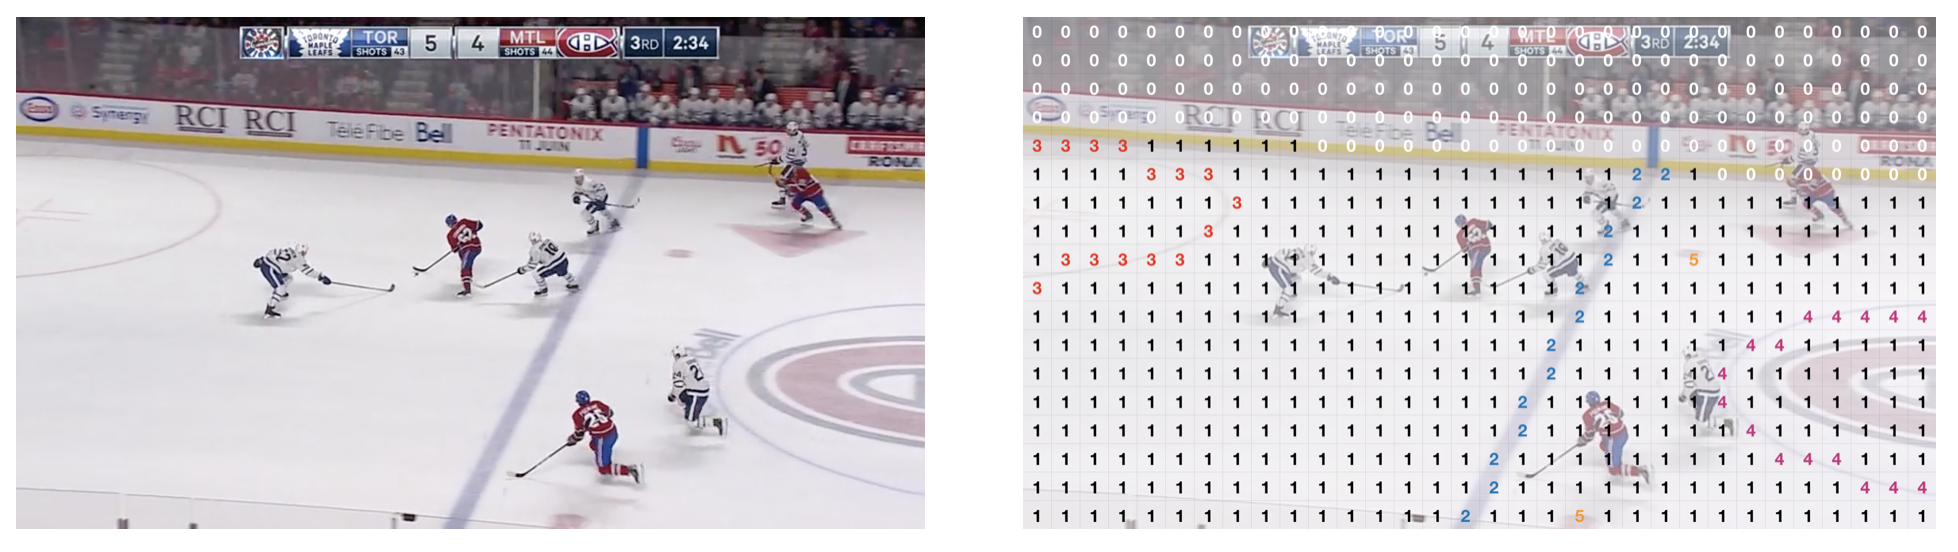
\includegraphics[width=1.0\linewidth]{figures/task-representation.png}}

We can summarize the workflow as follows where b is batch size and C is the number of classes:

\vspace{10mm}
{\centering 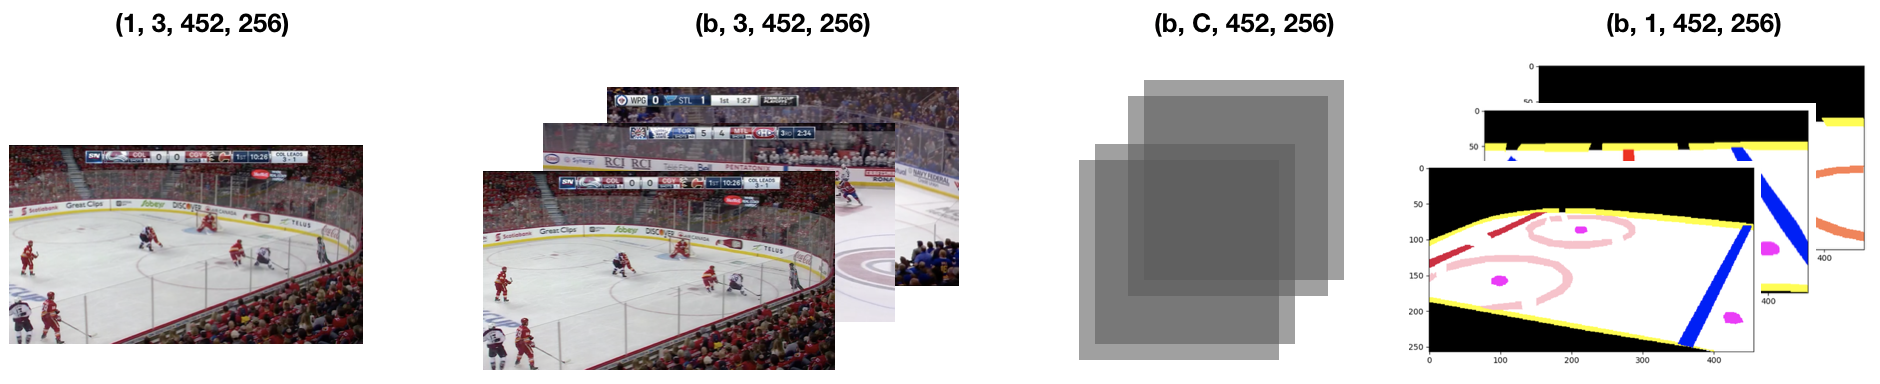
\includegraphics[width=45cm,height=10cm]{figures/dimensions.png}}


}	
\end{columns}











\begin{columns}

\column{.3}


% \block[bodyoffsety=48mm, titleoffsety=48mm]{Experiments}{
\block[bodyoffsety=0mm, titleoffsety=0mm]{Methodology}{
	
Our methodology is splitted in 3 main components:

\begin{enumerate}
	\item \textbf{Set up}
		\begin{itemize}
			\item Dataset creation
				\begin{itemize}
					\item 43 NHL broadcast images
				\end{itemize}
			\item Labeling task: \href{https://github.com/opencv/cvat}{cvat tool}
				\begin{itemize}
					\item 9 classes: crowd, ice, blue line, red line, goal line, circle zones, middle circle, dots and boards)
					\item 2 classes: crowd and ice
				\end{itemize}
		\end{itemize}
	\item \textbf{Semantic segmentation}
		\begin{itemize}
			\item Architecture set up
			\item Loss definition
			\item Data augmentation
			\item Training details
		\end{itemize}
	\item \textbf{Mapping to 2D plan}
		\begin{itemize}
			\item Key points recognition
			\item 2D translation
		\end{itemize}
\end{enumerate}


}


  \column{.7}
  \block[bodyoffsety=0mm, titleoffsety=0mm]{Architectures and training details}{
  	
  	\begin{multicols}{2}
  		\textbf{U-Net:} To perform our segmentation, we chose an architecture called U-Net. This network is \textbf{fast} and can be trained with \textbf{few images}. No pre-trained network found for that model.
  		
  		\vspace{10mm}
  		{\centering 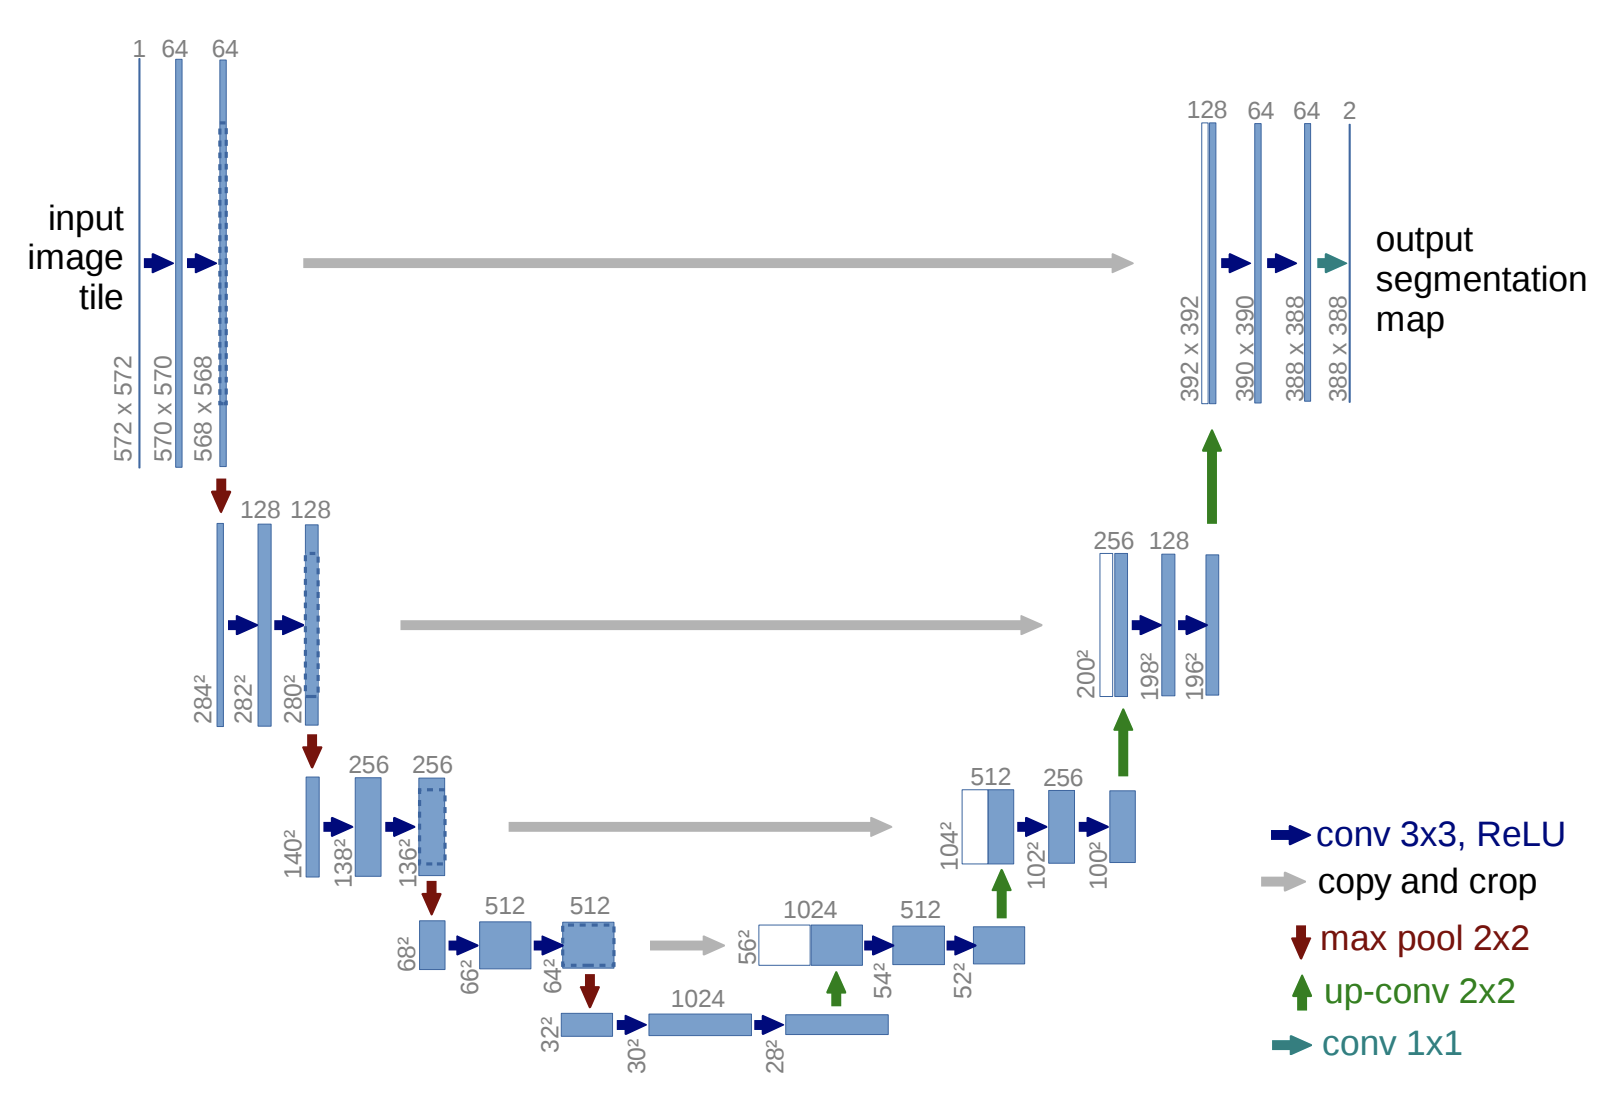
\includegraphics[width=1.0\linewidth]{figures/unet-architecture.png}}
  		
  		\textbf{VGG16:} We also decided to use a the 7 first layers of a \textbf{pre-trained} VGG16 architecture without the max-pooling steps. The resuting output we'll then the \textbf{same size} as the input.
  		  		
  		\columnbreak
  		
  		\textbf{Loss definition:} We defined 2 kinds of loss:
  		\begin{itemize}
  			\item Cross-Entropy loss
  			\item Dice loss
  		\end{itemize}
  	
		The 9-classes problem is suffering from \textbf{class imbalance} (there is much more pixels of ice/crowd than lines or dots. We address that problem in the dataset labeling and in the loss definition. For Cross-Entropy loss, we adapted the weights for loss depending on the label frequency. We also implemeted the Dice loss:
		
		  \vspace{-15mm}
		\begin{gather*}
			\text{Dice Loss} = \frac{1}{nb\_class}*\sum\limits_{i=1}^{nb\_class}\Big(1-\frac{2\sum\limits_{pixels}y_{true}y_{pred}}{\sum\limits_{pixels}y_{true}^{2}+\sum\limits_{pixels}y_{pred}^{2}}\Big)
		\end{gather*}
  		
  		\textbf{Training details:}
  		
  		\vspace{-10mm}
  		\begin{itemize}
  			\item Different learning rates (trainning schedule) and batch size
  			\item SGD optimizer with momentum and weight decay
  			\item Different upsampling methods (bilinear and transpose convolutions)
  		\end{itemize}
  		
  	\end{multicols}
  
  
  }
  




\end{columns}




















\begin{columns}

  \column{.4}


  \block{Dataset}{

  We created our own dataset by making screenshots of NHL broadcast games and labeled them. Here is an example of the after the labeling task (for both 9 classes (left) and 2 classes (right)):
  
  \vspace{5mm}
  {\centering 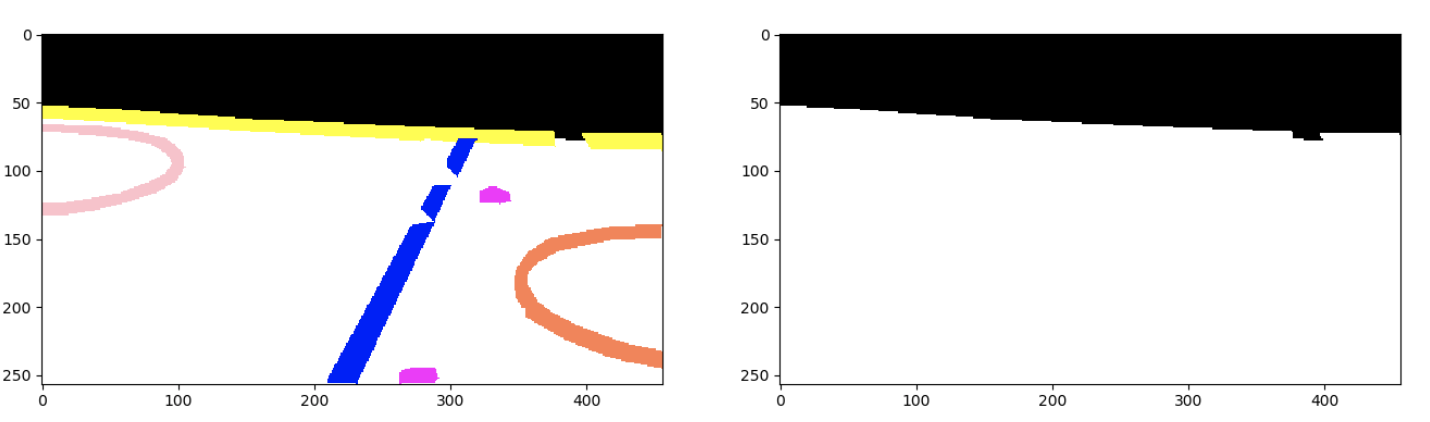
\includegraphics[width=30cm,height=8cm]{figures/example-labels.png}}
  
  To adress class imbalance, we draw larger areas around rare labels pixels such as dots, circles and lines.
  
  \vspace{1mm}
  
 Because we only had a total 43 images, we augmented our train dataset by making \textbf{horizontal rotation}. That kind of transformation makes sense in the context of a hockey ring (symmetry).
 
  \vspace{5mm}
 {\centering 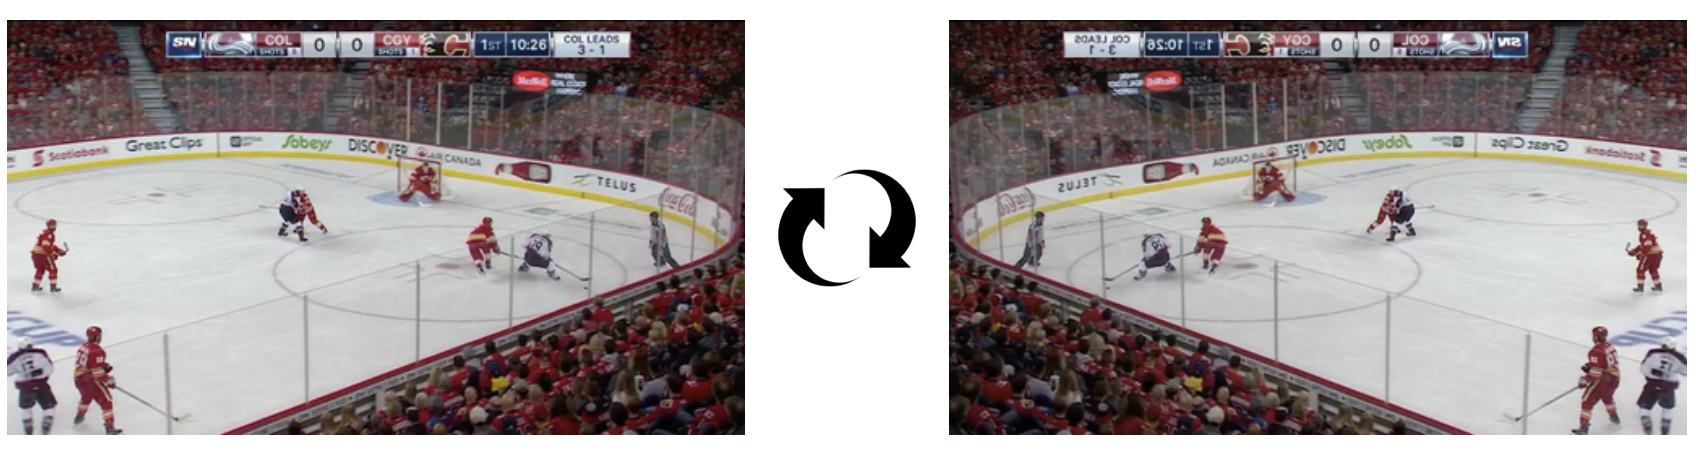
\includegraphics[width=30cm,height=8cm]{figures/rotation-example.png}}
 
   

  }









  \column{.38}
  \block{Results}
  {
  Here are the results we gathered from our best experiements:
  \begin{center}
  \setlength{\tabcolsep}{5mm}
  \begin{tabular}{c c c c c c}
  \toprule
  Labels & Model & Epochs & Loss & Train Loss & Valid Loss \\
  \midrule
  \multirow{2}{*}{9-classes} & U-Net & 210 & CE & 0.0962 &  \colorbold{0.2114} \\
  & VGG16 & 100 & Dice & 0.6810 & 0.7534 \\
  \midrule
  \multirow{1}{*}{2-classes} & U-Net  & 30 & CE  & 0.3471  & \colorbold{0.3788} \\
  \bottomrule
  \end{tabular}
  \end{center}
  
  \vspace{1mm}
  
  Here is sample that shows our best results for 9-classes U-Net model on test set images:
  
  \vspace{2mm}
  
  \begin{center}
  	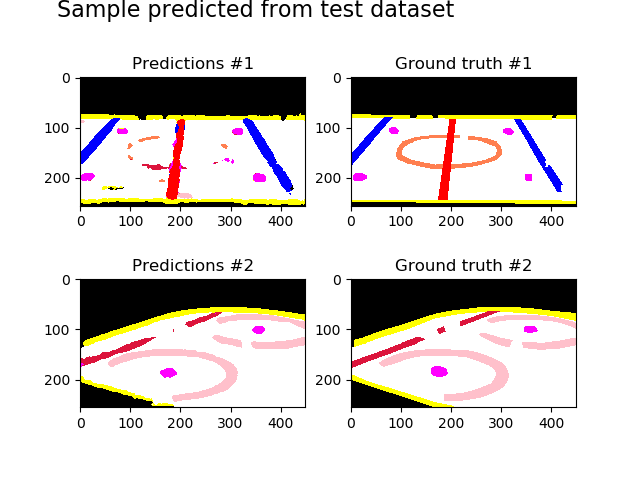
\includegraphics[width=25cm,height=16.2cm]{figures/test-new-model.png}
  \end{center}
  
  \vspace{-3mm}
  }







  
  
  
  \column{.22}
  
  
  \block{Conclusion}{
  
  \textbf{Discussion:}

    \begin{itemize}
        \item We don't need that much images (maybe specific to semantic segmentation)
        \item U-Net architecture generalizes well
        \item For 2-classes predictions, the performances are not enough good for the complexity of the problem.
    \end{itemize}
    
    \textbf{Future works:}

    \begin{itemize}
        \item Extract and label \textbf{more images} (was time consuming).
        \item Train a model to recognizes players on broadcast images
        \item Use the semantic segmentation learned by the model to map key areas on the ice into a \text{2D plan}.
        \vspace{5mm}
    \end{itemize}
  }

  
\end{columns}

\end{document}